% =============================================================================
% APPENDIX JJJ: METHOD-TRACKING - Intervention Registry
% =============================================================================
% Category: METHOD (Methodology)
% Version: 1.0
% Dependencies: Ch. 17-20, BBB (Parameters), EEE (Design), III (Cases)
% =============================================================================

\chapter{Intervention Registry: Learning Loop System}
\label{app:intervention-registry}

% -----------------------------------------------------------------------------
% METADATA BLOCK
% -----------------------------------------------------------------------------
\begin{tcolorbox}[colback=gray!5, colframe=gray!50, title=Appendix Metadata]
\begin{tabular}{ll}
\textbf{Code:} & JJJ \\
\textbf{Category:} & METHOD-TRACKING \\
\textbf{Purpose:} & Track predictions, results, and learnings for continuous improvement \\
\textbf{Data File:} & \texttt{data/intervention-registry.yaml} \\
\textbf{Query Tool:} & \texttt{scripts/query\_interventions.py} \\
\textbf{Slash Command:} & \texttt{/intervention} \\
\end{tabular}
\end{tcolorbox}

% -----------------------------------------------------------------------------
% FUNDAMENTAL QUESTION
% -----------------------------------------------------------------------------
\section{Fundamental Question}

\begin{tcolorbox}[colback=blue!5, colframe=blue!50, title=Central Question]
\textbf{How do we systematically learn from intervention projects to improve future predictions and designs?}
\end{tcolorbox}

The Intervention Registry implements a \textit{Learning Loop} that captures:
\begin{enumerate}
    \item \textbf{Ex-ante Predictions:} Expected effects per intervention and portfolio
    \item \textbf{Ex-post Results:} Actual measured outcomes
    \item \textbf{Deviation Analysis:} Systematic comparison with root cause identification
    \item \textbf{Parameter Updates:} Adjusted values for future predictions
    \item \textbf{Design Learnings:} Generalizable principles and recommendations
\end{enumerate}

% -----------------------------------------------------------------------------
% THE LEARNING LOOP
% -----------------------------------------------------------------------------
\section{The Learning Loop}

\subsection{Conceptual Framework}

\begin{figure}[h]
\centering
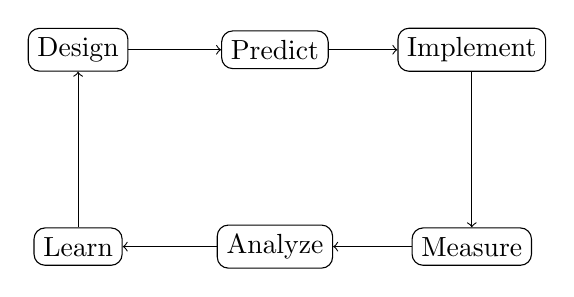
\begin{tikzpicture}[node distance=2.5cm, auto]
    \node[draw, rectangle, rounded corners] (design) {Design};
    \node[draw, rectangle, rounded corners, right of=design] (predict) {Predict};
    \node[draw, rectangle, rounded corners, right of=predict] (implement) {Implement};
    \node[draw, rectangle, rounded corners, below of=implement] (measure) {Measure};
    \node[draw, rectangle, rounded corners, left of=measure] (analyze) {Analyze};
    \node[draw, rectangle, rounded corners, left of=analyze] (learn) {Learn};

    \draw[->] (design) -- (predict);
    \draw[->] (predict) -- (implement);
    \draw[->] (implement) -- (measure);
    \draw[->] (measure) -- (analyze);
    \draw[->] (analyze) -- (learn);
    \draw[->] (learn) -- (design);
\end{tikzpicture}
\caption{The EBF Learning Loop}
\end{figure}

\subsection{Bayesian Parameter Update}

For each parameter $\theta$ (e.g., effect size for a default nudge), we update based on observations:

\begin{equation}
\theta_{new} = \frac{n_{lit} \cdot \theta_{lit} + n_{obs} \cdot \theta_{obs}}{n_{lit} + n_{obs}}
\end{equation}

Where:
\begin{itemize}
    \item $\theta_{lit}$ = literature-based parameter value
    \item $\theta_{obs}$ = observed value in project
    \item $n_{lit}$ = effective sample size from literature
    \item $n_{obs}$ = sample size of observation
\end{itemize}

% -----------------------------------------------------------------------------
% PROJECT STRUCTURE
% -----------------------------------------------------------------------------
\section{Project Data Structure}

\subsection{Seven Core Components}

Each project in the registry contains seven components:

\begin{table}[h]
\centering
\begin{tabular}{clp{7cm}}
\toprule
\textbf{\#} & \textbf{Component} & \textbf{Contents} \\
\midrule
1 & Meta & Name, client, domain, dates, status \\
2 & Context & Target behavior, population, baseline, segments \\
3 & Intervention Mix & List of interventions with $E_i$ predictions \\
4 & Complementarity Matrix & $\gamma_{ij}$ for all intervention pairs \\
5 & Predictions & Portfolio effect $E(P)$, KPI predictions \\
6 & Results & Actual KPI values, measured effects \\
7 & Deviation Analysis & Comparison, root causes, learnings \\
\bottomrule
\end{tabular}
\caption{Project Data Components}
\end{table}

\subsection{Intervention Entry Schema}

\begin{verbatim}
intervention:
  id: "I1"
  type: nudge|incentive|information|commitment|social|environmental
  subtype: default|labeling|gamification|...
  description: "What the intervention does"
  timing: "When in the journey"
  target_segment: all|segment_name
  parameters:
    intensity: 0.0-1.0
    duration: "time period"
    frequency: "how often"
  expected_contribution:
    E_i: float          # predicted effect
    confidence: float   # 0-1
    source: literature|pilot|expert
\end{verbatim}

\subsection{Deviation Entry Schema}

\begin{verbatim}
deviation_analysis:
  overall:
    predicted_E_P: float
    actual_E_P: float
    delta: float
    delta_pct: float
    direction: overestimate|accurate|underestimate
  by_intervention:
    - id: "I1"
      predicted: float
      actual: float
      delta: float
      likely_causes: [string]
  root_causes:
    - cause: "Description"
      evidence: "Supporting data"
      confidence: high|medium|low
\end{verbatim}

% -----------------------------------------------------------------------------
% PREDICTION FORMULA
% -----------------------------------------------------------------------------
\section{Portfolio Effect Prediction}

The registry uses the portfolio effect formula from Chapter 20:

\begin{equation}
E(P) = \sum_{i} E_i + \sum_{i<j} \gamma_{ij} \cdot \sqrt{E_i \cdot E_j}
\end{equation}

With confidence intervals calculated as:

\begin{equation}
CI = E(P) \pm z_{\alpha/2} \cdot \sqrt{\sum_i \sigma^2_{E_i} + \sum_{i<j} \sigma^2_{\gamma_{ij}}}
\end{equation}

\subsection{Confidence Mapping}

\begin{table}[h]
\centering
\begin{tabular}{lcc}
\toprule
\textbf{Source} & \textbf{Typical Confidence} & \textbf{Effective n} \\
\midrule
Literature (meta-analysis) & 0.80-0.95 & 1000+ \\
Literature (single study) & 0.60-0.80 & 100-500 \\
Pilot study & 0.40-0.70 & 50-200 \\
Expert estimate & 0.30-0.50 & 10-50 \\
\bottomrule
\end{tabular}
\caption{Confidence Levels by Source}
\end{table}

% -----------------------------------------------------------------------------
% DEVIATION ANALYSIS PROTOCOL
% -----------------------------------------------------------------------------
\section{Deviation Analysis Protocol}

\subsection{Step 1: Calculate Overall Deviation}

\begin{equation}
\Delta = E(P)_{actual} - E(P)_{predicted}
\end{equation}

\begin{equation}
\Delta\% = \frac{\Delta}{E(P)_{predicted}} \times 100
\end{equation}

\subsection{Step 2: Attribution by Intervention}

For each intervention $i$, estimate $E_i^{actual}$ through:
\begin{itemize}
    \item Controlled comparison (if available)
    \item Time-series analysis (intervention timing)
    \item Expert judgment with uncertainty
\end{itemize}

\subsection{Step 3: Root Cause Analysis}

Systematic investigation of:
\begin{enumerate}
    \item \textbf{Context factors:} Was $\Psi$ different than assumed?
    \item \textbf{Segment distribution:} Were proportions different?
    \item \textbf{Implementation fidelity:} Was intervention as designed?
    \item \textbf{Interaction effects:} Were $\gamma_{ij}$ values wrong?
    \item \textbf{Parameter values:} Were $E_i$ estimates wrong?
\end{enumerate}

\subsection{Step 4: Confidence-Weighted Learning}

\begin{equation}
\text{Learning Weight} = \frac{n \cdot \text{attribution\_confidence}}{\sum n \cdot \text{attribution\_confidence}}
\end{equation}

% -----------------------------------------------------------------------------
% AGGREGATED LEARNINGS
% -----------------------------------------------------------------------------
\section{Aggregated Learnings}

The registry automatically aggregates learnings across projects:

\subsection{DACH Context Adjustments}

Based on observed systematic deviations from US/UK literature values:

\begin{table}[h]
\centering
\begin{tabular}{lcccc}
\toprule
\textbf{Parameter} & \textbf{Literature} & \textbf{DACH Observed} & \textbf{Factor} & \textbf{n} \\
\midrule
Default Effect & 0.35 & 0.42 & 1.20 & 1 \\
Social Norm Feedback & 0.020 & 0.018 & 0.90 & 1 \\
Gamification (Adults) & 0.06 & 0.03 & 0.50 & 1 \\
\bottomrule
\end{tabular}
\caption{DACH Context Adjustments (as of Version 1.0)}
\end{table}

\subsection{Design Principles Derived}

From project learnings, the following principles emerged:

\begin{enumerate}
    \item \textbf{Max 3 visible interventions:} More triggers perceived manipulation (PRJ-002)
    \item \textbf{Gamification segmentation:} Only for extrinsically motivated (PRJ-002)
    \item \textbf{DACH cultural adjustment:} Apply 0.9-1.2× factors to US literature (multiple)
\end{enumerate}

\subsection{Segment Insights}

\begin{table}[h]
\centering
\begin{tabular}{lp{5cm}cc}
\toprule
\textbf{Segment} & \textbf{Insight} & \textbf{$\sigma_{lit}$} & \textbf{$\sigma_{obs}$} \\
\midrule
rational-calculative & Skeptisch bei Defaults, bevorzugt Argumentation & 0.8 & 0.6 \\
present-biased & Stärkere Response auf Defaults in DACH & 1.5 & 1.9 \\
\bottomrule
\end{tabular}
\caption{Segment-Specific $\sigma$ Adjustments}
\end{table}

% -----------------------------------------------------------------------------
% QUERY INTERFACE
% -----------------------------------------------------------------------------
\section{Query Interface}

\subsection{Project Queries}

\begin{verbatim}
/intervention PRJ-001         # Specific project
/intervention --domain health # By domain
/intervention --status active # By status
/intervention --list          # All projects
\end{verbatim}

\subsection{Analysis Queries}

\begin{verbatim}
/intervention --deviation     # Deviation analysis
/intervention --learnings     # All learnings
/intervention --parameters    # Parameter updates
/intervention --accuracy      # Prediction accuracy
\end{verbatim}

% -----------------------------------------------------------------------------
% INTEGRATION
% -----------------------------------------------------------------------------
\section{Integration with EBF Components}

\begin{table}[h]
\centering
\begin{tabular}{lll}
\toprule
\textbf{Phase} & \textbf{EBF Component} & \textbf{Integration} \\
\midrule
Design & EEE (METHOD-DESIGN) & Use workflow for intervention mix \\
Parameters & BBB (CORE-WHERE) & Pull $E_i$, $\gamma_{ij}$ values \\
Cases & III (REF-CASES) & Find similar past cases \\
Prediction & Ch. 20 & Apply portfolio formula \\
Learnings & BBB update & Push revised parameters \\
\bottomrule
\end{tabular}
\caption{Registry Integration Points}
\end{table}

% -----------------------------------------------------------------------------
% QUALITY METRICS
% -----------------------------------------------------------------------------
\section{Quality Metrics}

\subsection{Prediction Accuracy Tracking}

\begin{equation}
\text{MAPE} = \frac{1}{n} \sum_{i=1}^{n} \left| \frac{E(P)_i^{pred} - E(P)_i^{actual}}{E(P)_i^{actual}} \right|
\end{equation}

Target: MAPE $< 25\%$ after 10+ projects

\subsection{Learning Velocity}

\begin{equation}
\text{Learning Velocity} = \frac{\Delta \text{MAPE}}{\Delta \text{projects}}
\end{equation}

Target: Negative (improving accuracy with each project)

% -----------------------------------------------------------------------------
% REFERENCES
% -----------------------------------------------------------------------------
\section{References}

\subsection{Technical Implementation}
\begin{itemize}
    \item Registry Data: \texttt{data/intervention-registry.yaml}
    \item Query Script: \texttt{scripts/query\_interventions.py}
    \item Slash Command: \texttt{.claude/commands/intervention.md}
\end{itemize}

\subsection{Related Appendices}
\begin{itemize}
    \item Case Library: III (REF-CASES)
    \item Model Design: EEE (METHOD-DESIGN)
    \item Parameters: BBB (CORE-WHERE)
    \item Chapter 17-20: Intervention System
\end{itemize}

\nocite{bcm_master}

\end{chapter}
